\section{APPENDIX: MC closure Check}
\label{sec:MCclosureCheck}

To perform the MC closure check, the pseudodata samples are prepared to mimic each of the data samples needed for the fit. This includes (1) W$\gamma$ samples to be used for fit (full analysis selection without $I_{ch}$ or $\sigma_{i\eta i\eta}$ cuts), those samples are prepared separately for the muon and electron channels; (2) W$\gamma$ in full selection to be plotted into the [data vs bkg+signal] plots, separately for the two channels; (3) Z$\gamma$ FSR selected sample for the real-$\gamma$ templates, muon and electron channles are merged; (4) Z$\gamma$+DYjets ISR selected sample for the fake-$\gamma$ templates, channels are merged. To prepare the pseudodata W$\gamma$ samples, the W$\gamma$, Wjets, Z$\gamma$, DYjets, tt$\gamma$, ttjets, and WW$\gamma$ MC samples were merged with the W$\gamma$ selection applied. To prepare the pseudodata Z$\gamma$ samples, the Z$\gamma$ and DYjets MC samples were merged with the appropriate Z$\gamma$ selections applied. Luminosity normalizations, PU and scale factor weights are applied on these MC samples.\\   
Then the pseudodata are treated as if they were data to perform the fits, prepare the plots and subtract the background. All the MC samples used in the actual analysis with data are used with the analysis with the pseudodata the same way.\\

\begin{figure}[htb]
  \begin{center}
   \includegraphics[width=0.33\textwidth]{figs_v11/MUON_WGamma/PrepareYields/c_TotalDATAvsMC_Barrel__phoEt.png}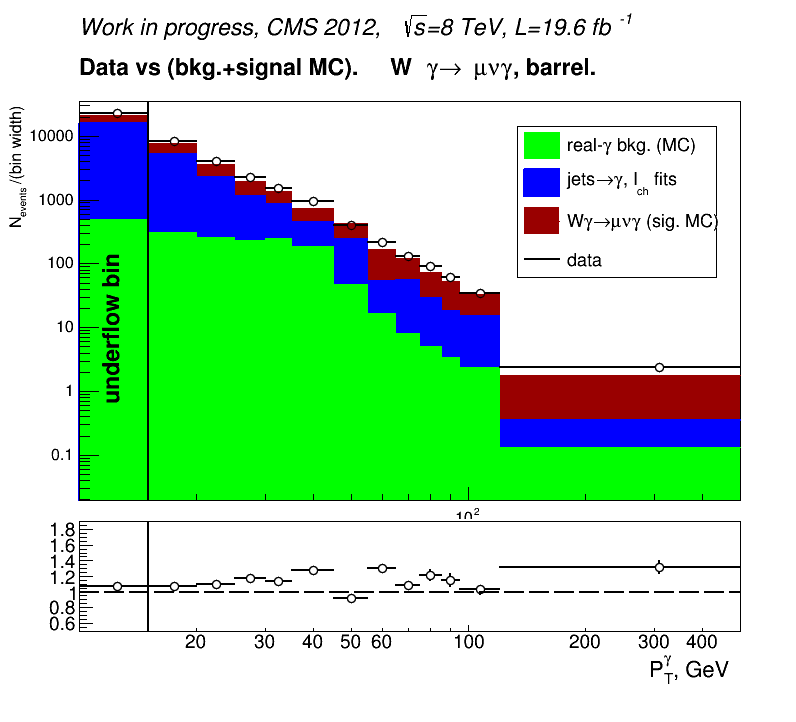
\includegraphics[width=0.33\textwidth]{figs_v11/MUON_WGamma/PrepareYields/c_DATAvsBkgPlusSigMCc_MUON_WGamma_TEMPL_CHISO_UNblind__Barrel__phoEt.png}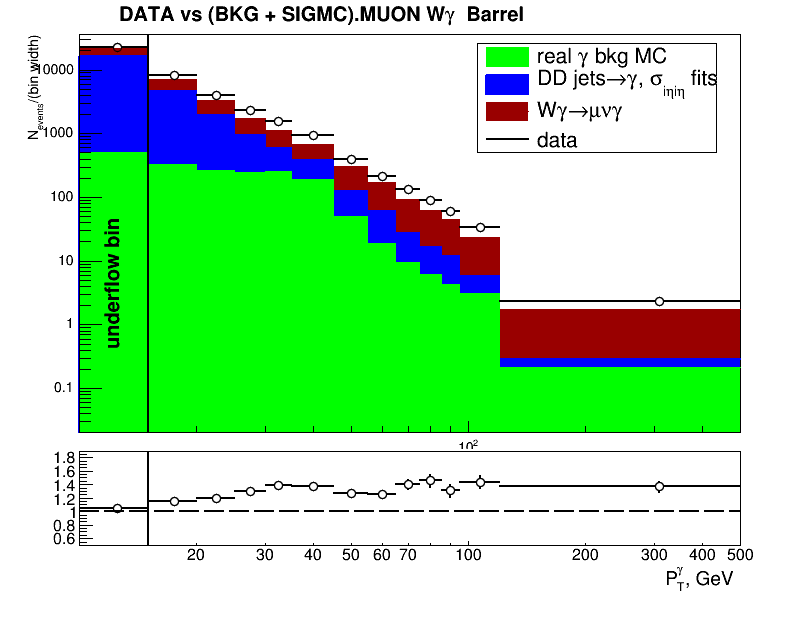
\includegraphics[width=0.33\textwidth]{figs_v11/MUON_WGamma/PrepareYields/c_DATAvsBkgPlusSigMCc_MUON_WGamma_TEMPL_SIHIH_UNblind__Barrel__phoEt.png}
   \includegraphics[width=0.33\textwidth]{figs_v11/MUON_WGamma/PrepareYields/c_TotalDATAvsMC_Barrel__phoEt_MCclosure.png}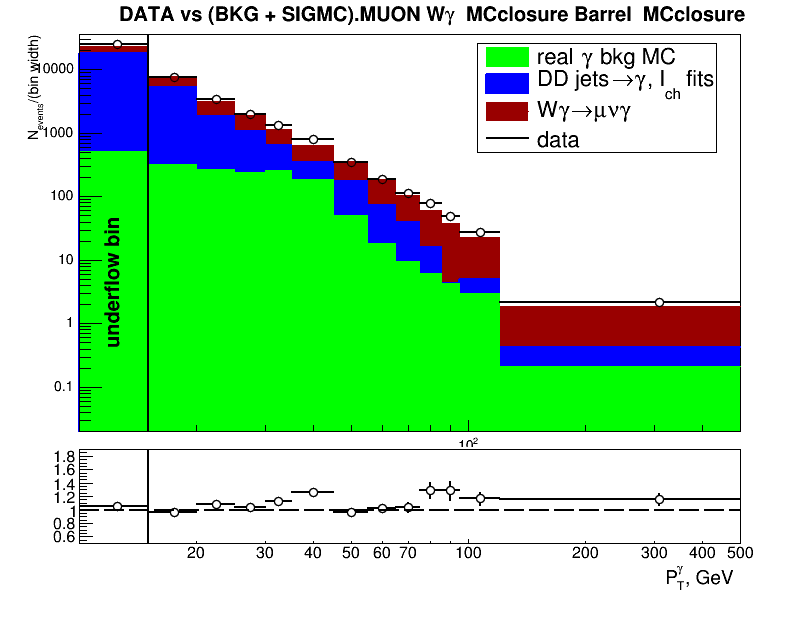
\includegraphics[width=0.33\textwidth]{figs_v11/MUON_WGamma/PrepareYields/c_DATAvsBkgPlusSigMCc_MUON_WGamma_TEMPL_CHISO_UNblind_MCclosure__Barrel__phoEt_MCclosure.png}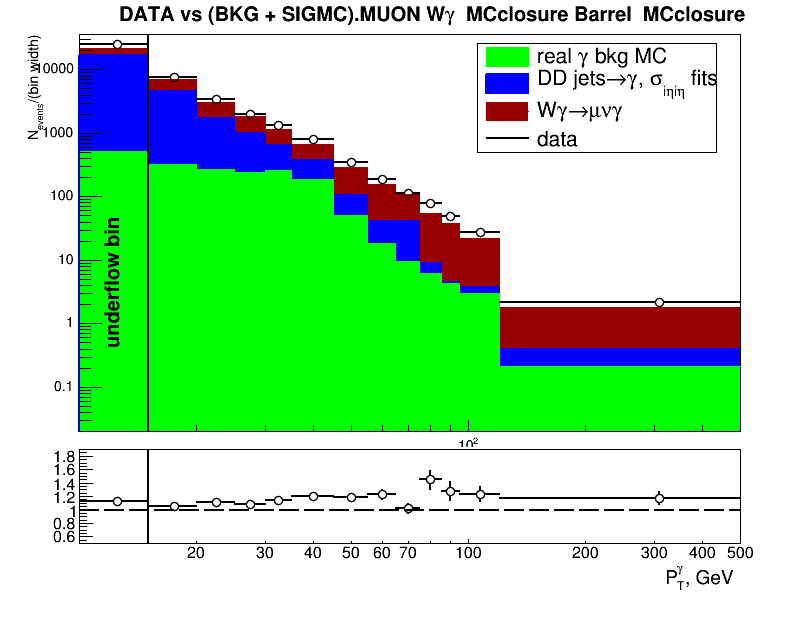
\includegraphics[width=0.33\textwidth]{figs_v11/MUON_WGamma/PrepareYields/c_DATAvsBkgPlusSigMCc_MUON_WGamma_TEMPL_SIHIH_UNblind_MCclosure__Barrel__phoEt_MCclosure.png}
  \caption{DD estimates in bins of phoEt. Muon Barrel. Top: data, bottom: MC-closure. }
  \end{center}
\end{figure}

\begin{figure}[htb]
  \begin{center}
   \includegraphics[width=0.33\textwidth]{figs_v11/MUON_WGamma/PrepareYields/c_TotalDATAvsMC_Endcap__phoEt.png}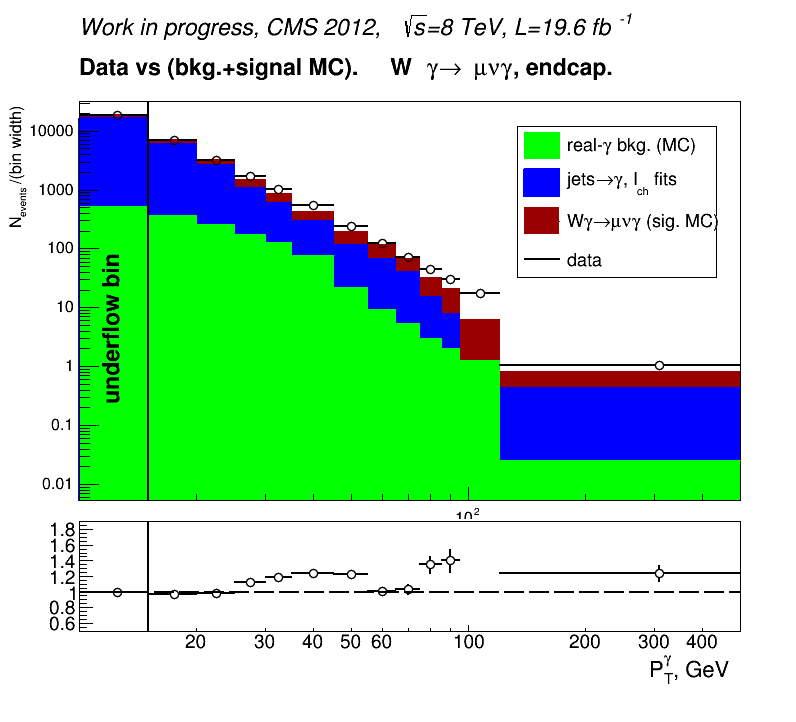
\includegraphics[width=0.33\textwidth]{figs_v11/MUON_WGamma/PrepareYields/c_DATAvsBkgPlusSigMCc_MUON_WGamma_TEMPL_CHISO_UNblind__Endcap__phoEt.png}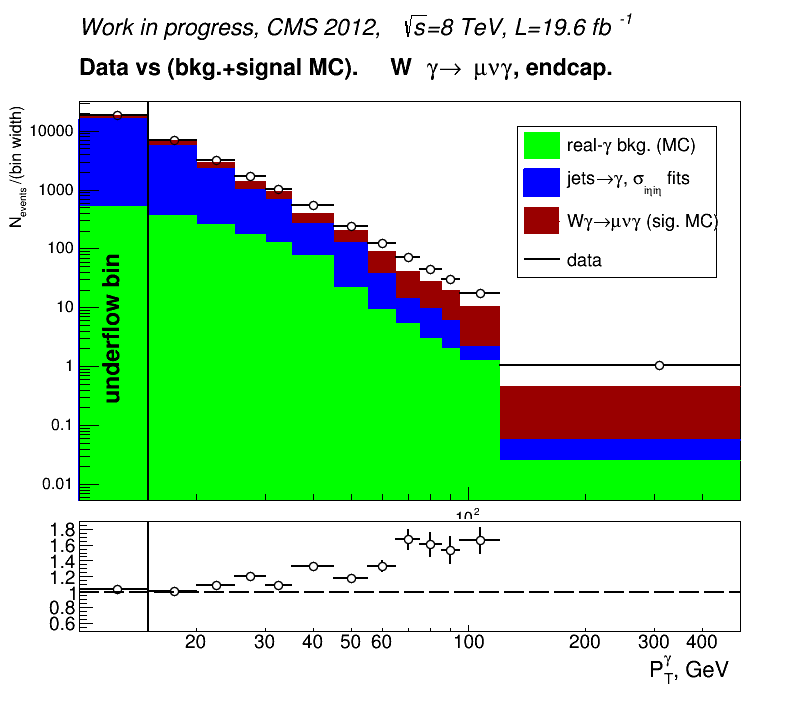
\includegraphics[width=0.33\textwidth]{figs_v11/MUON_WGamma/PrepareYields/c_DATAvsBkgPlusSigMCc_MUON_WGamma_TEMPL_SIHIH_UNblind__Endcap__phoEt.png}
   \includegraphics[width=0.33\textwidth]{figs_v11/MUON_WGamma/PrepareYields/c_TotalDATAvsMC_Endcap__phoEt_MCclosure.png}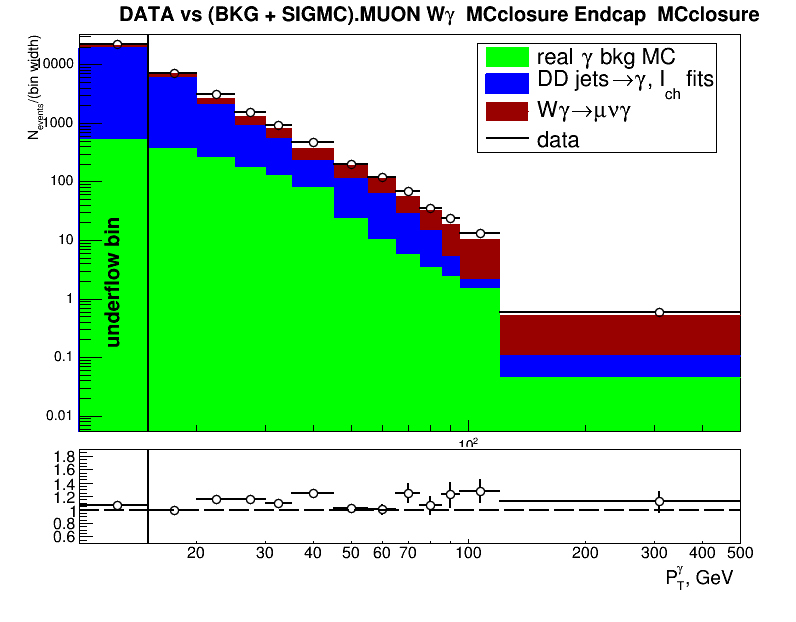
\includegraphics[width=0.33\textwidth]{figs_v11/MUON_WGamma/PrepareYields/c_DATAvsBkgPlusSigMCc_MUON_WGamma_TEMPL_CHISO_UNblind_MCclosure__Endcap__phoEt_MCclosure.png}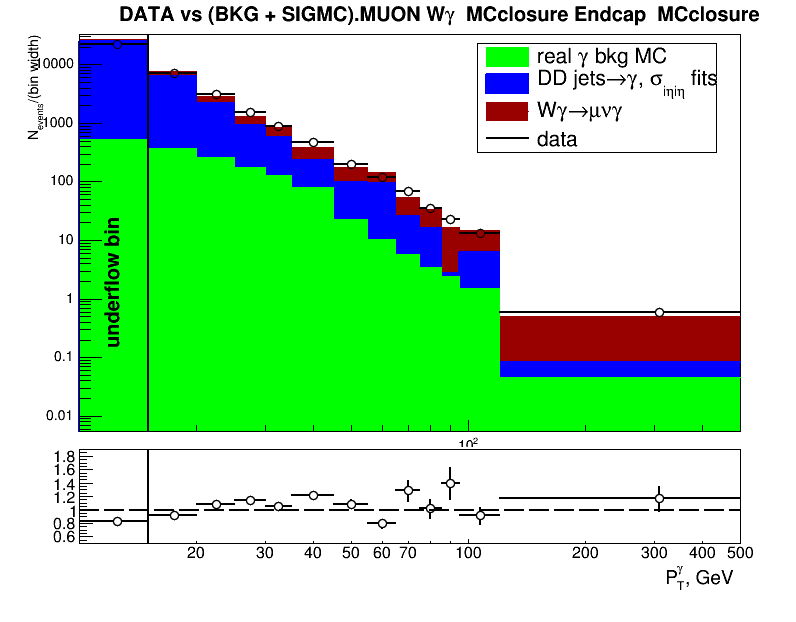
\includegraphics[width=0.33\textwidth]{figs_v11/MUON_WGamma/PrepareYields/c_DATAvsBkgPlusSigMCc_MUON_WGamma_TEMPL_SIHIH_UNblind_MCclosure__Endcap__phoEt_MCclosure.png}
  \caption{DD estimates in bins of phoEt. Muon Endcap. Top: data, bottom: MC-closure.}
  \end{center}
\end{figure}

\begin{figure}[htb]
  \begin{center}
   \includegraphics[width=0.33\textwidth]{figs_v11/ELECTRON_WGamma/PrepareYields/c_TotalDATAvsMC_Barrel__phoEt.png}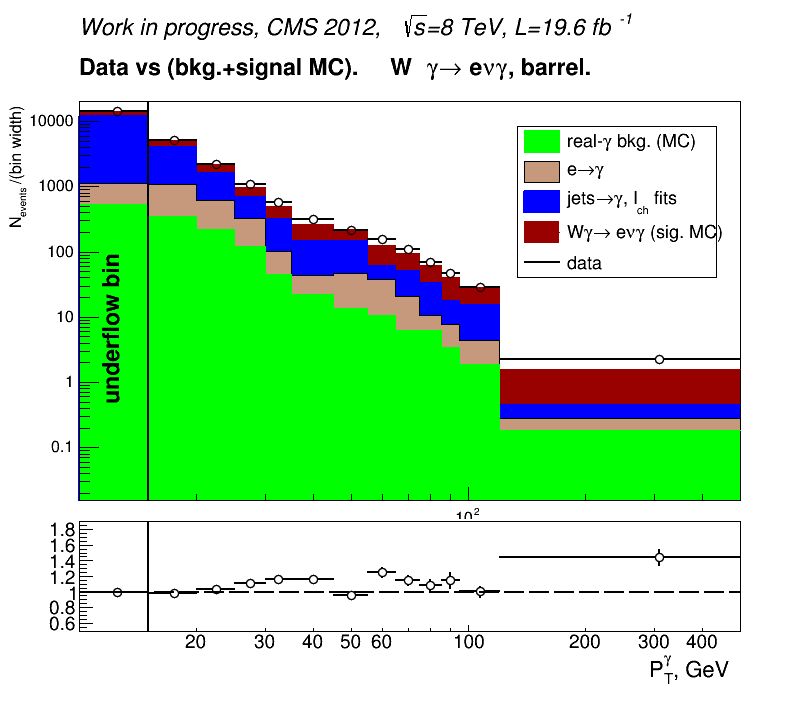
\includegraphics[width=0.33\textwidth]{figs_v11/ELECTRON_WGamma/PrepareYields/c_DATAvsBkgPlusSigMCc_ELECTRON_WGamma_TEMPL_CHISO_UNblind__Barrel__phoEt.png}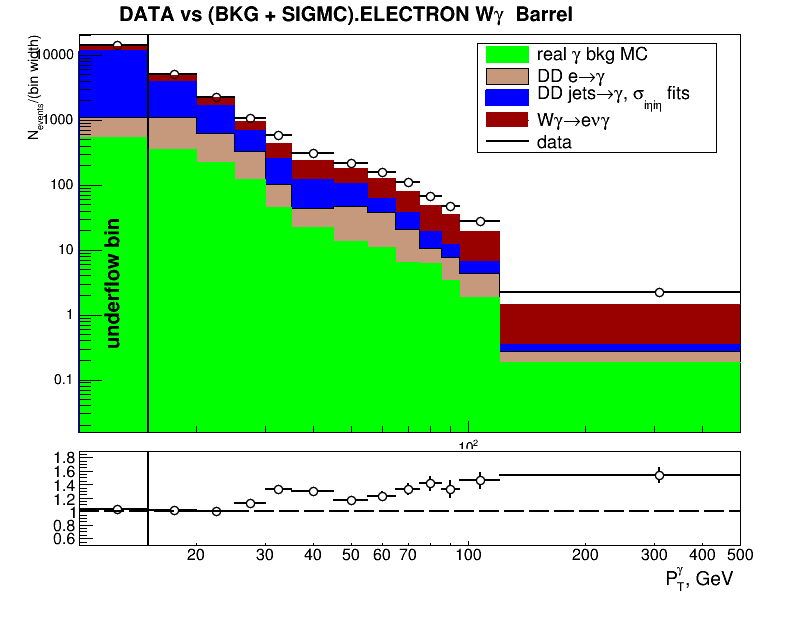
\includegraphics[width=0.33\textwidth]{figs_v11/ELECTRON_WGamma/PrepareYields/c_DATAvsBkgPlusSigMCc_ELECTRON_WGamma_TEMPL_SIHIH_UNblind__Barrel__phoEt.png}
   \includegraphics[width=0.33\textwidth]{figs_v11/ELECTRON_WGamma/PrepareYields/c_TotalDATAvsMC_Barrel__phoEt_MCclosure.png}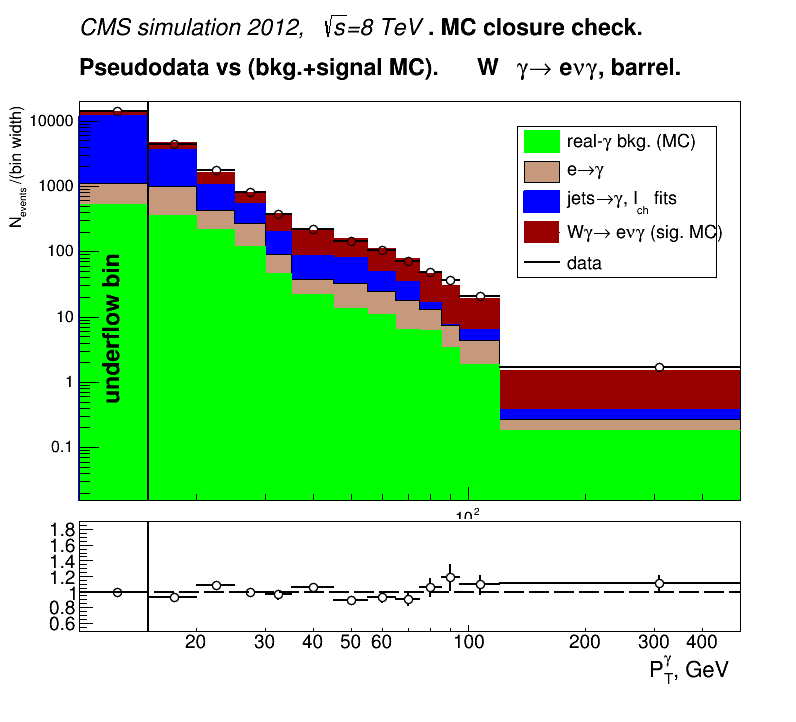
\includegraphics[width=0.33\textwidth]{figs_v11/ELECTRON_WGamma/PrepareYields/c_DATAvsBkgPlusSigMCc_ELECTRON_WGamma_TEMPL_CHISO_UNblind_MCclosure__Barrel__phoEt_MCclosure.png}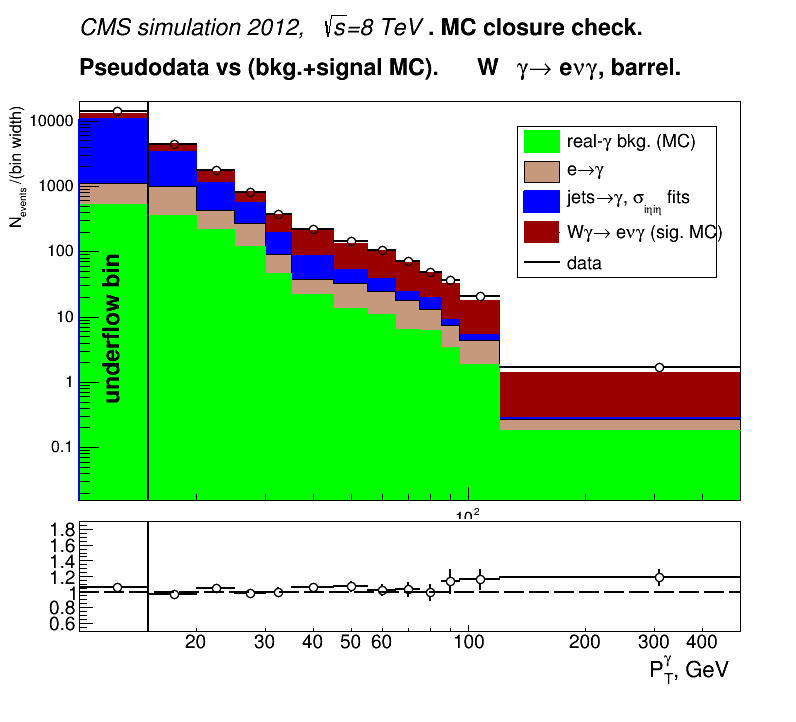
\includegraphics[width=0.33\textwidth]{figs_v11/ELECTRON_WGamma/PrepareYields/c_DATAvsBkgPlusSigMCc_ELECTRON_WGamma_TEMPL_SIHIH_UNblind_MCclosure__Barrel__phoEt_MCclosure.png}
  \caption{DD estimates in bins of phoEt. Muon Barrel. Top: data, bottom: MC-closure. }
  \end{center}
\end{figure}

\begin{figure}[htb]
  \begin{center}
   \includegraphics[width=0.33\textwidth]{figs_v11/ELECTRON_WGamma/PrepareYields/c_TotalDATAvsMC_Endcap__phoEt.png}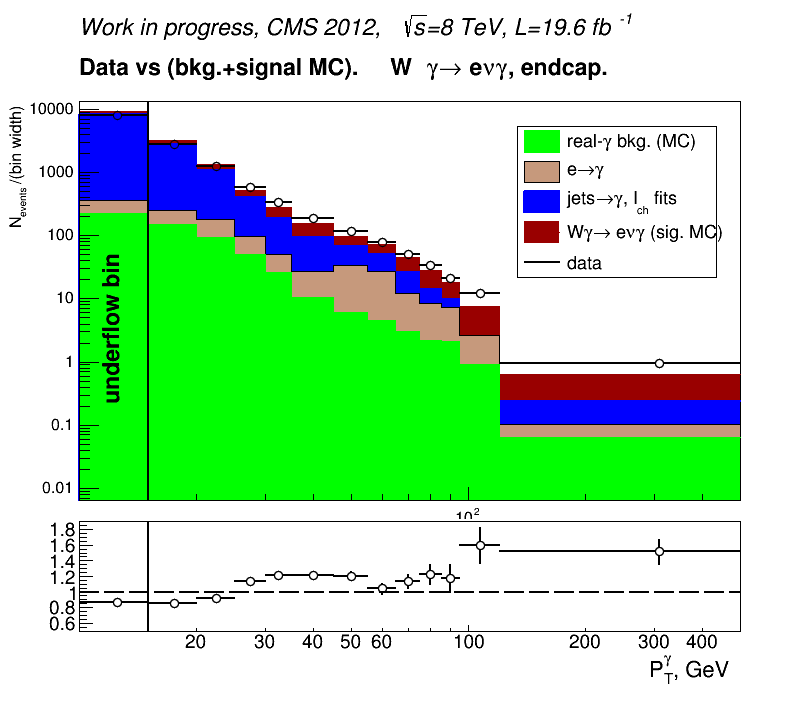
\includegraphics[width=0.33\textwidth]{figs_v11/ELECTRON_WGamma/PrepareYields/c_DATAvsBkgPlusSigMCc_ELECTRON_WGamma_TEMPL_CHISO_UNblind__Endcap__phoEt.png}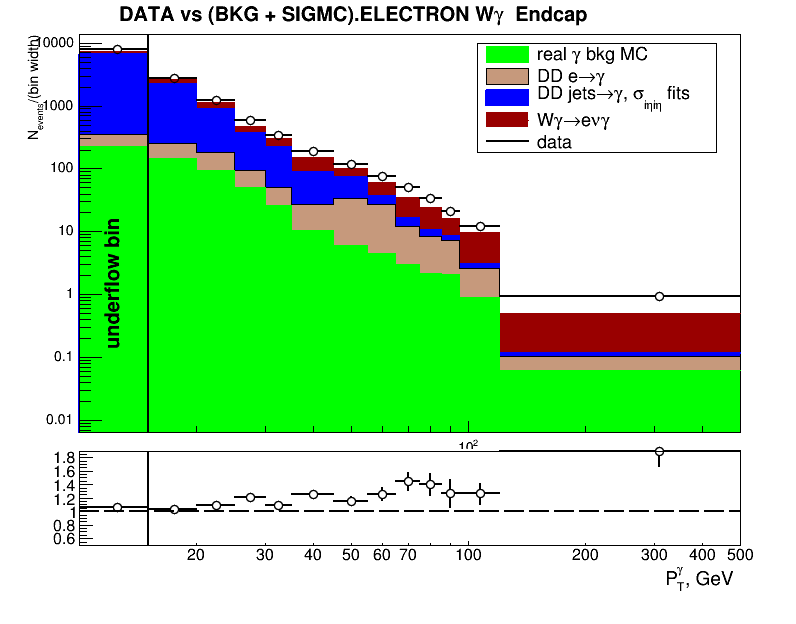
\includegraphics[width=0.33\textwidth]{figs_v11/ELECTRON_WGamma/PrepareYields/c_DATAvsBkgPlusSigMCc_ELECTRON_WGamma_TEMPL_SIHIH_UNblind__Endcap__phoEt.png}
   \includegraphics[width=0.33\textwidth]{figs_v11/ELECTRON_WGamma/PrepareYields/c_TotalDATAvsMC_Endcap__phoEt_MCclosure.png}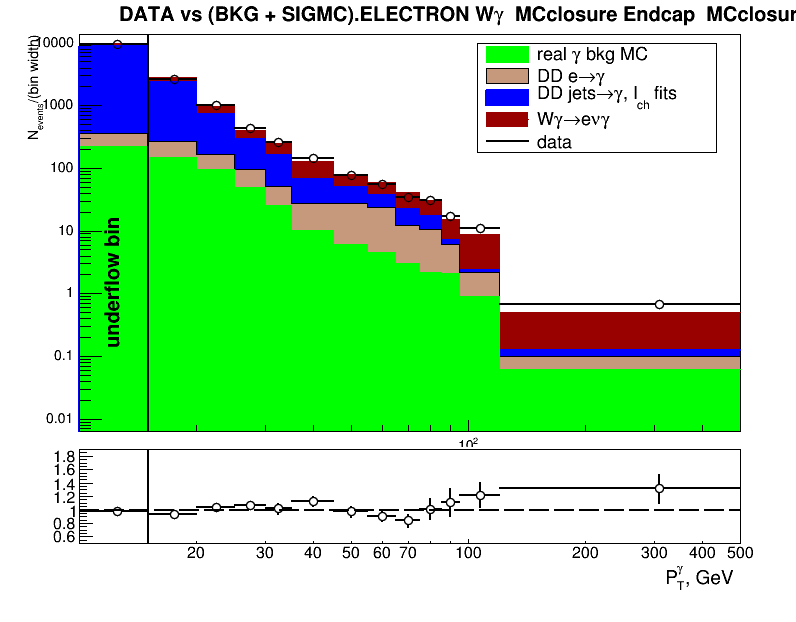
\includegraphics[width=0.33\textwidth]{figs_v11/ELECTRON_WGamma/PrepareYields/c_DATAvsBkgPlusSigMCc_ELECTRON_WGamma_TEMPL_CHISO_UNblind_MCclosure__Endcap__phoEt_MCclosure.png}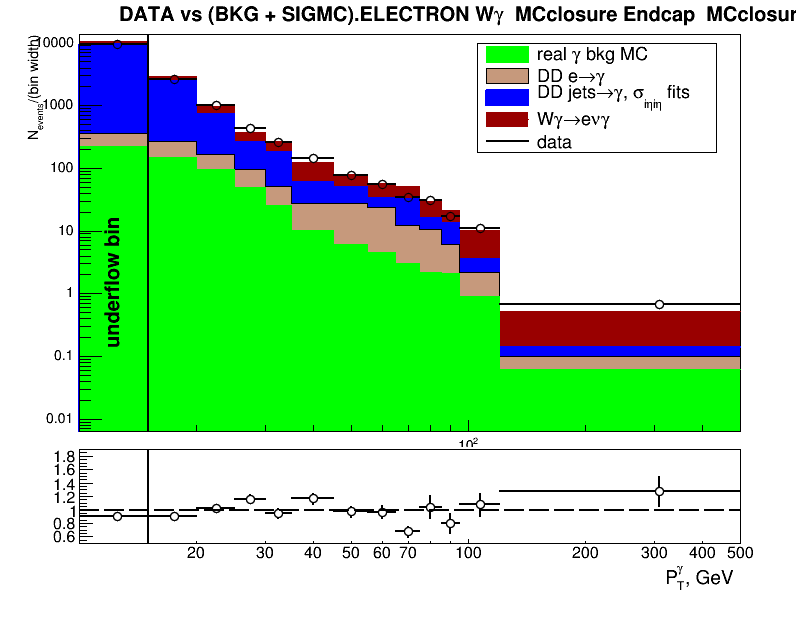
\includegraphics[width=0.33\textwidth]{figs_v11/ELECTRON_WGamma/PrepareYields/c_DATAvsBkgPlusSigMCc_ELECTRON_WGamma_TEMPL_SIHIH_UNblind_MCclosure__Endcap__phoEt_MCclosure.png}
  \caption{DD estimates in bins of phoEt. Muon Endcap. Top: data, bottom: MC-closure.}
  \end{center}
\end{figure}
